\documentclass{article}
\usepackage{babel}
\usepackage[utf8]{inputenc}    % Codificación UTF-8 para acentos y caracteres especiales
\usepackage[T1]{fontenc}       % Soporte de tipografía
\usepackage{babel}[spanish]    % Soporte para español


% ---------------------------
% Márgenes y diseño de página
% ---------------------------
\usepackage[a4paper, left=3cm, right=2.5cm, top=3cm, bottom=3cm]{geometry} % Márgenes
\usepackage{amsmath}
\usepackage{amsfonts}
\usepackage{graphicx}
\usepackage{hyperref}
\usepackage{algorithm}
\usepackage{algorithmic}
\usepackage{listings}
\usepackage{xcolor}

\lstset{
    language=Python,
    basicstyle=\ttfamily\small,
    keywordstyle=\color{blue},
    commentstyle=\color{gray},
    stringstyle=\color{red},
    showstringspaces=false,
    breaklines=true,
    frame=single,
    captionpos=b
}



\title{Integraci\'on Num\'erica con el M\'etodo \texttt{quad} y Cambios de Variable en Integrales Improprias}
\author{}
\date{}

\begin{document}

\maketitle

\section{Introducción}
La integración numérica de funciones en intervalos infinitos o con comportamientos singulares requiere t\'ecnicas especiales. Una de las herramientas más utilizadas en Python es la función \texttt{quad} de SciPy, basada en los algoritmos de QUADPACK, una biblioteca de 

\section{Funcionamiento del Método \texttt{quad}}
\subsection{Introducción}
La cuadratura de Gauss-Kronrod es una extensión de la cuadratura de Gauss que permite estimar simultáneamente la integral de una función y el error de la aproximación. Se basa en agregar nodos adicionales a los nodos de Gauss para obtener una evaluación más precisa de la integral.

\subsection{Cómo funciona}
Partimos de una cuadratura de Gauss con $n$ nodos, que es exacta para polinomios de grado hasta $2n-1$. La extensi\'on de Kronrod introduce $2n+1$ nodos en total, incluyendo los $n$ nodos originales de Gauss, y es exacta para polinomios de grado hasta $3n+1$ aproximadamente.

El método Gauss-Kronrod utiliza los mismos nodos de Gauss más nodos adicionales intercalados. Esto permite calcular dos aproximaciones de la integral:
\begin{itemize}
    \item Una aproximación de orden más bajo (Gauss).
    \item Una aproximación de orden más alto (Kronrod).
\end{itemize}

Comparando estas dos aproximaciones, se estima el error local de la integral sobre un subintervalo dado. Si el error es mayor que una tolerancia dada, se subdivide el intervalo y se repite el procedimiento.

\subsection{¿Por qué funciona?}
La clave está en que la cuadratura de Gauss proporciona una estimación muy eficiente para funciones suaves, y la extensión de Kronrod mejora dicha estimación sin requerir evaluaciones adicionales de la función en los nodos ya existentes.

Además, al calcular dos integrales de diferente orden de exactitud, podemos estimar el error de la integral de manera efectiva sin necesitar información adicional sobre la derivada de la función.

\subsection{Pseudocódigo y código en Python}
El Pseudocódigo del algoritmo de integración adaptativa Gauss-Kronrod es el siguiente:
\begin{algorithm}[H]
\caption{Integración adaptativa Gauss-Kronrod}
\begin{algorithmic}[1]
\STATE \textbf{Entrada:} Función $f$, intervalo $[a,b]$, tolerancias $\varepsilon_{\text{abs}}$, $\varepsilon_{\text{rel}}$
\STATE Inicializar pila de intervalos con $[a,b]$
\STATE Inicializar $\text{total} \leftarrow 0$
\WHILE{pila no vacía}
    \STATE Extraer intervalo $[a_1,b_1]$
    \STATE Calcular $I_G$ (integral Gauss) y $I_K$ (integral Kronrod) en $[a_1,b_1]$
    \STATE Calcular error estimado $e = |I_G - I_K|$
    \STATE Calcular tolerancia local $\tau = \max(\varepsilon_{\text{abs}}, \varepsilon_{\text{rel}} \times |I_K|)$
    \IF{$e < \tau$}
        \STATE $\text{total} \leftarrow \text{total} + I_K$
    \ELSE
        \STATE Subdividir intervalo en dos partes
        \STATE Agregar ambos subintervalos a la pila
    \ENDIF
\ENDWHILE
\STATE \textbf{Salida:} $\text{total}$
\end{algorithmic}
\end{algorithm}

Su implementación en python puede encontrarse en el archivo adjunto y en la siguiente sección. 

\subsection{Implementación en Python}
\begin{lstlisting}[caption={Implementación de la integración adaptativa con cuadratura Gauss-Kronrod}]
    import numpy as np #Aunque no es necesario, se recomienda importar numpy para el manejo de arrays y funciones matematicas.
    import warnings # Para manejar advertencias de convergencia
    
    # Valores para cuadratura de Gauss-Kronrod 10-21 puntos (G10-K21) oficiales
    xgauss = np.array([
        -9.739065285171717200779640120844521e-01,
        -8.650633666889845107320966884234930e-01,
        -6.794095682990244062343273651148736e-01,
        -4.333953941292471907992659431657842e-01,
        -1.488743389816312108848260011297200e-01,
        1.488743389816312108848260011297200e-01,
        4.333953941292471907992659431657842e-01,
        6.794095682990244062343273651148736e-01,
        8.650633666889845107320966884234930e-01,
        9.739065285171717200779640120844521e-01
    ])

    wgauss = np.array([
        6.667134430868813759356880989333179e-02,
        1.494513491505805931457763396576973e-01,
        2.190863625159820439955349342281632e-01,
        2.692667193099963550912269215694694e-01,
        2.955242247147528701738929946513383e-01,
        2.955242247147528701738929946513383e-01,
        2.692667193099963550912269215694694e-01,
        2.190863625159820439955349342281632e-01,
        1.494513491505805931457763396576973e-01,
        6.667134430868813759356880989333179e-02
    ])

    xkronrod = np.array([
        -9.956571630258080807355272806890028e-01,
        -9.739065285171717200779640120844521e-01,
        -9.301574913557082260012071800595083e-01,
        -8.650633666889845107320966884234930e-01,
        -7.808177265864168970637175783450424e-01,
        -6.794095682990244062343273651148736e-01,
        -5.627571346686046833390000992726941e-01,
        -4.333953941292471907992659431657842e-01,
        -2.943928627014601981311266031038656e-01,
        -1.488743389816312108848260011297200e-01,
        0.000000000000000000000000000000000e+00,
        1.488743389816312108848260011297200e-01,
        2.943928627014601981311266031038656e-01,
        4.333953941292471907992659431657842e-01,
        5.627571346686046833390000992726941e-01,
        6.794095682990244062343273651148736e-01,
        7.808177265864168970637175783450424e-01,
        8.650633666889845107320966884234930e-01,
        9.301574913557082260012071800595083e-01,
        9.739065285171717200779640120844521e-01,
        9.956571630258080807355272806890028e-01
    ])

    wkronrod = np.array([
        1.169463886737187427806439606219205e-02,
        3.255816230796472747881897245938976e-02,
        5.475589657435199603138130024458018e-02,
        7.503967481091995276704314091619001e-02,
        9.312545458369760553506546508336634e-02,
        1.093871588022976418992105903258050e-01,
        1.234919762620658510779581098310742e-01,
        1.347092173114733259280540017717068e-01,
        1.427759385770600807970942731387171e-01,
        1.477391049013384913748415159720680e-01,
        1.494455540029169056649364683898212e-01,
        1.477391049013384913748415159720680e-01,
        1.427759385770600807970942731387171e-01,
        1.347092173114733259280540017717068e-01,
        1.234919762620658510779581098310742e-01,
        1.093871588022976418992105903258050e-01,
        9.312545458369760553506546508336634e-02,
        7.503967481091995276704314091619001e-02,
        5.475589657435199603138130024458018e-02,
        3.255816230796472747881897245938976e-02,
        1.169463886737187427806439606219205e-02
    ])
        
    def gauss_kronrod(f, a, b):
        mid = 0.5 * (a + b)
        half_length = 0.5 * (b - a)
    
        nodes = mid + half_length * xkronrod
        f_nodes = f(nodes)
        integral = half_length * np.sum(wkronrod * f_nodes)
    
        nodes_gauss = mid + half_length * xgauss
        f_nodes_gauss = f(nodes_gauss)
        integral_gauss = half_length * np.sum(wgauss * f_nodes_gauss)
    
        error_estimate = np.abs(integral - integral_gauss)
    
        return integral, error_estimate
    
    def adaptive_integrate(f, a, b, epsabs=1e-15, epsrel=1e-15, limit=10000, record_intervals=True):
        if np.isinf(a) or np.isinf(b):
            if np.isinf(a) and not np.isinf(b): #Manejo de limites infinitos mediante el cambio de variable
                g = lambda t: f(t/(1-t)) * (1 / (1-t)**2)
                return adaptive_integrate(g, 0.0, 1 , epsabs, epsrel, limit)
            elif not np.isinf(a) and np.isinf(b):
                g = lambda t: f(t/(1-t)) * (1 / (1-t)**2)
                return adaptive_integrate(g, 0.0, 1 , epsabs, epsrel, limit)
            else:
                raise ValueError("Cannot integrate from -inf to +inf with this mapping.")
    
        stack = [(a, b)]
        total = 0.0
        iterations = 0
        
        intervals = [(a, b)]  # Para almacenar los intervalos evaluados
        while stack:
            iterations += 1
            if iterations > limit:
                warnings.warn("Too many iterations, adding last evaluated interval.")
                a1, b1 = stack.pop()
                integral, _ = gauss_kronrod(f, a1, b1)
                total += integral
                break
    
            a1, b1 = stack.pop()
            if a1 == b1:
                continue
    
            integral, error = gauss_kronrod(f, a1, b1)
            tolerance = max(epsabs, epsrel * np.abs(integral))
    
            if np.isnan(error) or np.isnan(integral):
                continue
    
            if error < tolerance:
                total += integral
            else:
                mid = 0.5 * (a1 + b1)
                stack.append((mid, b1))
                stack.append((a1, mid))
                if record_intervals:
                    intervals.append((a1, mid))
                    intervals.append((mid, b1))
    
        if record_intervals:
            print("Intervalos evaluados:", intervals)
            print("Numero de intervalos:", len(intervals))
            print("Numero de iteraciones:", iterations)
            return total, intervals
        else:
            return total
    \end{lstlisting}



\section{Cambio de Variable para Intervalos Infinitos}
Uno de los problemas más comunes en la integración numérica es el tratamiento de las integrales impropias. Una de las técnicas mas utilizadas es tener en cuenta la biyección de la semirrecta $[0, \infty)$ con el intervalo $[0, 1]$. Esto permite transformar la integral impropia en una integral definida en un intervalo finito. Dicha biyección viene dada por:

\begin{equation}
    x = \frac{t}{1-t}, \quad t \in (0,1).
    \label{eq:biyeccion}
\end{equation}
    
Como vemos, $x$ toma todos los valores de $[0, \infty)$ cuando $t$ varía de $0$ a $1$. La diferencial asociada a este cambio de variable es, 
\[
    dx = \frac{1}{(1-t)^2} dt.
\]
De modo que:
\[
    \int_0^{\infty} f(x) \, dx = \int_0^1 f\left(\frac{t}{1-t}\right) \frac{dt}{(1-t)^2}.
\]
Como se ha comentado en reuniones anteriores, el cambio de variable propuesto aquí no es el único (aunque sí parece el más extendido en las diferentes bibliotecas que se han comentado), aunque en general parecen mejorar la precisión de la integración. También existe la posibilidad de programar este método a mano, aumentando el número de puntos y nodos de la integración. Sin embargo, esto puede ser más costoso computacionalmente y no siempre es necesario. En este caso, se ha optado por utilizar la función \texttt{quad} de SciPy, que ya implementa este cambio de variable de manera interna.

\section{Resultados Numéricos}
En el estudio práctico se analizaron funciones de dos tipos. Las primeras de tipo exponencial*potencia son funciones "similares" a las que encontramos en la construcción de las densidades atómicas. Estudiaremos el caso, 
\begin{equation}
    f(x) = N x^a e^{-bx}, \quad x \in [0, \infty), \quad a > -1, \quad b > 0 \quad a, b \in \mathbb{R},
\end{equation}
con $N$ una constante de normalización $N = \frac{b^{a+1}}{\Gamma(a+1)}$, donde $\Gamma$ es la función gamma. Aunque las distribuciones de probabilidad reales de los átomos (sobretodo de los más pesados) tienen una estructura más rica que esta función, aquí nos limitamos a estudiar la convergencia de la integral impropia en el intervalo $[0, \infty)$, que es el que nos interesa.

Por otro lado, se estudian funciones de tipo potencia que decaen muy lentamente a infinito, mucho más lentamente de lo que decaen las funciones anteriores. Aquí solamente queremos "forzar la maquina" ver  En este caso, se estudia la función:
\[
    f(x) = \frac{p-1}{(1+x)^p}, \quad p > 1
\]
que decaen lentamente a infinito. Se realizaron integraciones:
\begin{itemize}
    \item Sin cambio de variable.
    \item Con cambio de variable.
    \item Usando \texttt{trapz}, \texttt{quad} y \texttt{fixed\_quad}.
\end{itemize}

\subsection{Resultados para la función $f(x) = N x^a e^{-bx}$}

Como vemos es una funcion $f(x) = N x e^{-0.01x}$ que decae relativamente rápido a infinito. Es algo similar al tipo de funciones con las que se construyen las bases de Slater. Como era de esperar, el método \texttt{quad} proporciona resultados muy precisos a la integral de esta función (recordemos que el método \texttt{quad} realiza el cambio de variable (\ref{eq:biyeccion}) de forma automática). Algo más sorprendente es el método \texttt{trapz},  que proporciona los segundos mejores resultados en este cálculo cuando se aplica el cambio de variable mencionado en \ref{eq:biyeccion}. Sin embargo, el metodo \texttt{fixed\_quad} proporciona de los peores resultados (y aun peores resultados cuando realizamos el cambio de variable). Esto puede deberse a las dificultades que tiene el método quad para evaluar cerca de singularidades, de ahí que la función sin transformar proporcione mejores resultados.

\begin{table}[h!]
    \centering
    \begin{tabular}{|l|c|c|c|}
    \hline
    \textbf{Método} & \textbf{Resultado} & \textbf{Error absoluto} & \textbf{Tiempo (s)} \\
    \hline
    Adaptativo (propio) & 1.000000000000001 & $1 \times 10^{-15}$ & 0.000687 \\
    quad                & 1.000000000000000 & $0$                 & 0.000223 \\
    trapz (0--100)       & 0.999500517388558 & $4.9948 \times 10^{-4}$ & 0.000037 \\
    trapz (cambio var)   & 0.999999999999800 & $2.00 \times 10^{-13}$  & 0.000021 \\
    fixed\_quad (0--100) & 0.999500600772616 & $4.9939 \times 10^{-4}$ & 0.000023 \\
    fixed\_quad (cambio var) & 1.038522182629414 & $3.8522 \times 10^{-2}$ & 0.000014 \\
    \hline
    \end{tabular}
    \caption{Comparación de precisión y rendimiento entre distintos métodos de integración para $f(x) = \frac{0.01^{2}}{\Gamma(2)} x e^{-0.01x}$}
    \label{tab:resultados_exponencial}
\end{table}
Graficar las funciones nos puede ayudar a enter los resultados expuestos en la tabla. 
\begin{figure}
    \centering
    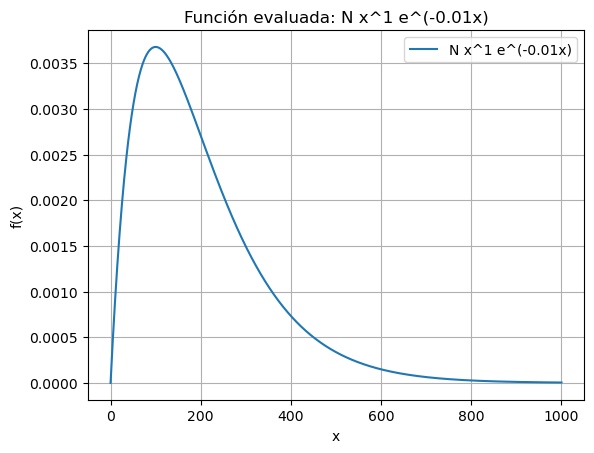
\includegraphics[width=0.8\textwidth]{figures/f_prueba_exp.png}
    \caption{Comparación de la función $f(x) = N x^a e^{-bx}$ $[0, 1000]$}
    \label{fig:gauss_kronrod}
\end{figure}

El método adaptativo realizado por mi proporciona resultados similares al método \texttt{quad}, aunque algo más lentos. Esto se debe a que el método \texttt{quad} utiliza menos puntos de Gauss-Kronrod en intervalos infinitos (al hacer el cambio de variable). Además de que \texttt{quad} es más rápido que el método adaptado por mi, también es más preciso debido a procesos internos mucho más optimizados que los usados por mí. Digamos que \texttt{quad} tiene la mejor relación precisión/velocidad.

\subsection{Resultados para la función $f(x) = \frac{p-1}{(1+x)^p}$}

\begin{table}[H]
    \centering
    \begin{tabular}{|l|c|c|c|}
    \hline
    \textbf{Método} & \textbf{Resultado} & \textbf{Error absoluto} & \textbf{Tiempo (s)} \\
    \hline
    Adaptativo (propio) & 0.924142187135658 & $0.075857812864342$ & 0.206181 \\
    
    \texttt{quad} & 1.000000000000013 & $0.000000000000013$ & 0.000101 \\
    
    \texttt{trapz} (0--100) & 0.498954443499032 & $0.501045556500968$ & 0.000069 \\
    
    \texttt{trapz} (cambio var) & 0.776819826552289 & $0.223180173447711$ & 0.000038 \\
    
    \texttt{fixed\_quad} (0--100) & 0.497723532253270 & $0.502276467746730$ & 0.000236 \\
    
    \texttt{fixed\_quad} (cambio var) & 0.596396468056625 & $ 0.403603531943375$ & 0.000023 \\
    \hline
    \end{tabular}
    \caption{Comparación de métodos de integración numérica para una función de tipo potencia lenta.}
    \label{tab:resultados_potencia}
\end{table}
    
Como vemos esta función "lleva al límite" a todas las funciones de integración, la única con capacidad de converger es el método \texttt{quad}.

\begin{figure}
    \centering
    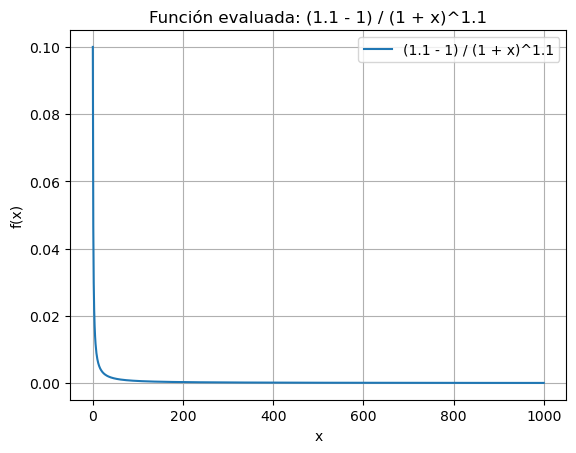
\includegraphics[width=0.8\textwidth]{figures/f_prueba_ld.png}
    \caption{Comparación de la función $f(x) = \frac{p-1}{(1+x)^p}$ $[0, 100]$}
    \label{fig:gauss_kronrod}
\end{figure}


\section{Conclusiones}
El método \texttt{quad} proporciona integración precisa gracias a su adaptabilidad y al cambio de variable automático en intervalos infinitos. Como vemos para este tipo de funciones, es importante realizar un estudio previo y bien, identificar que método es mejor para cada función hacer intervalos de integración "personalizados" para la función dada.

El método \texttt{quad} es el más adaptable (valga la redundancia) a todas las situaciones, pero es cierto que puede llegar a requerir más tiempo de computación que otros métodos. Tal vez, se podría investigar el uso del método \texttt{trapz} con el cambio de variable, pues parece obtener resultados muy similares a los de \texttt{quad} para este tipo de funciones en mucho menos tiempo (cabe mencionar que el tiempo de \texttt{quad} es bastante más variable que el de \texttt{trapz} pues depende de cuantas subdivisiones se hagan en todo el proceso). 

\end{document}

